\section{Dati a disposizione} \label{dati-a-disposizione}
Per validare l'architettura proposta dal progetto PANTHEON gli autori dello stesso hanno preso in considerazione un vero noccioleto su cui effettuare le sperimentazioni. Il noccioleto in questione appartiene all'\textit{Azienda Agricola Vignola}, una impresa agricola situata nel comune di Caprarola, in provincia di Viterbo.\par

In particolare, ai fini della sperimentazione del progetto PANTHEON, sono stati presi in considerazione 3 appezzamenti di terreno di proprieta dell'Azienda Agricola Vignola. Dei 3 appezzamenti, solo 2 sono stati poi effettivamente impiegati per effettuare i test (field 16 e 18 nella figura \ref{fig:selectedfields}).

\begin{figure}[ht]
\centering
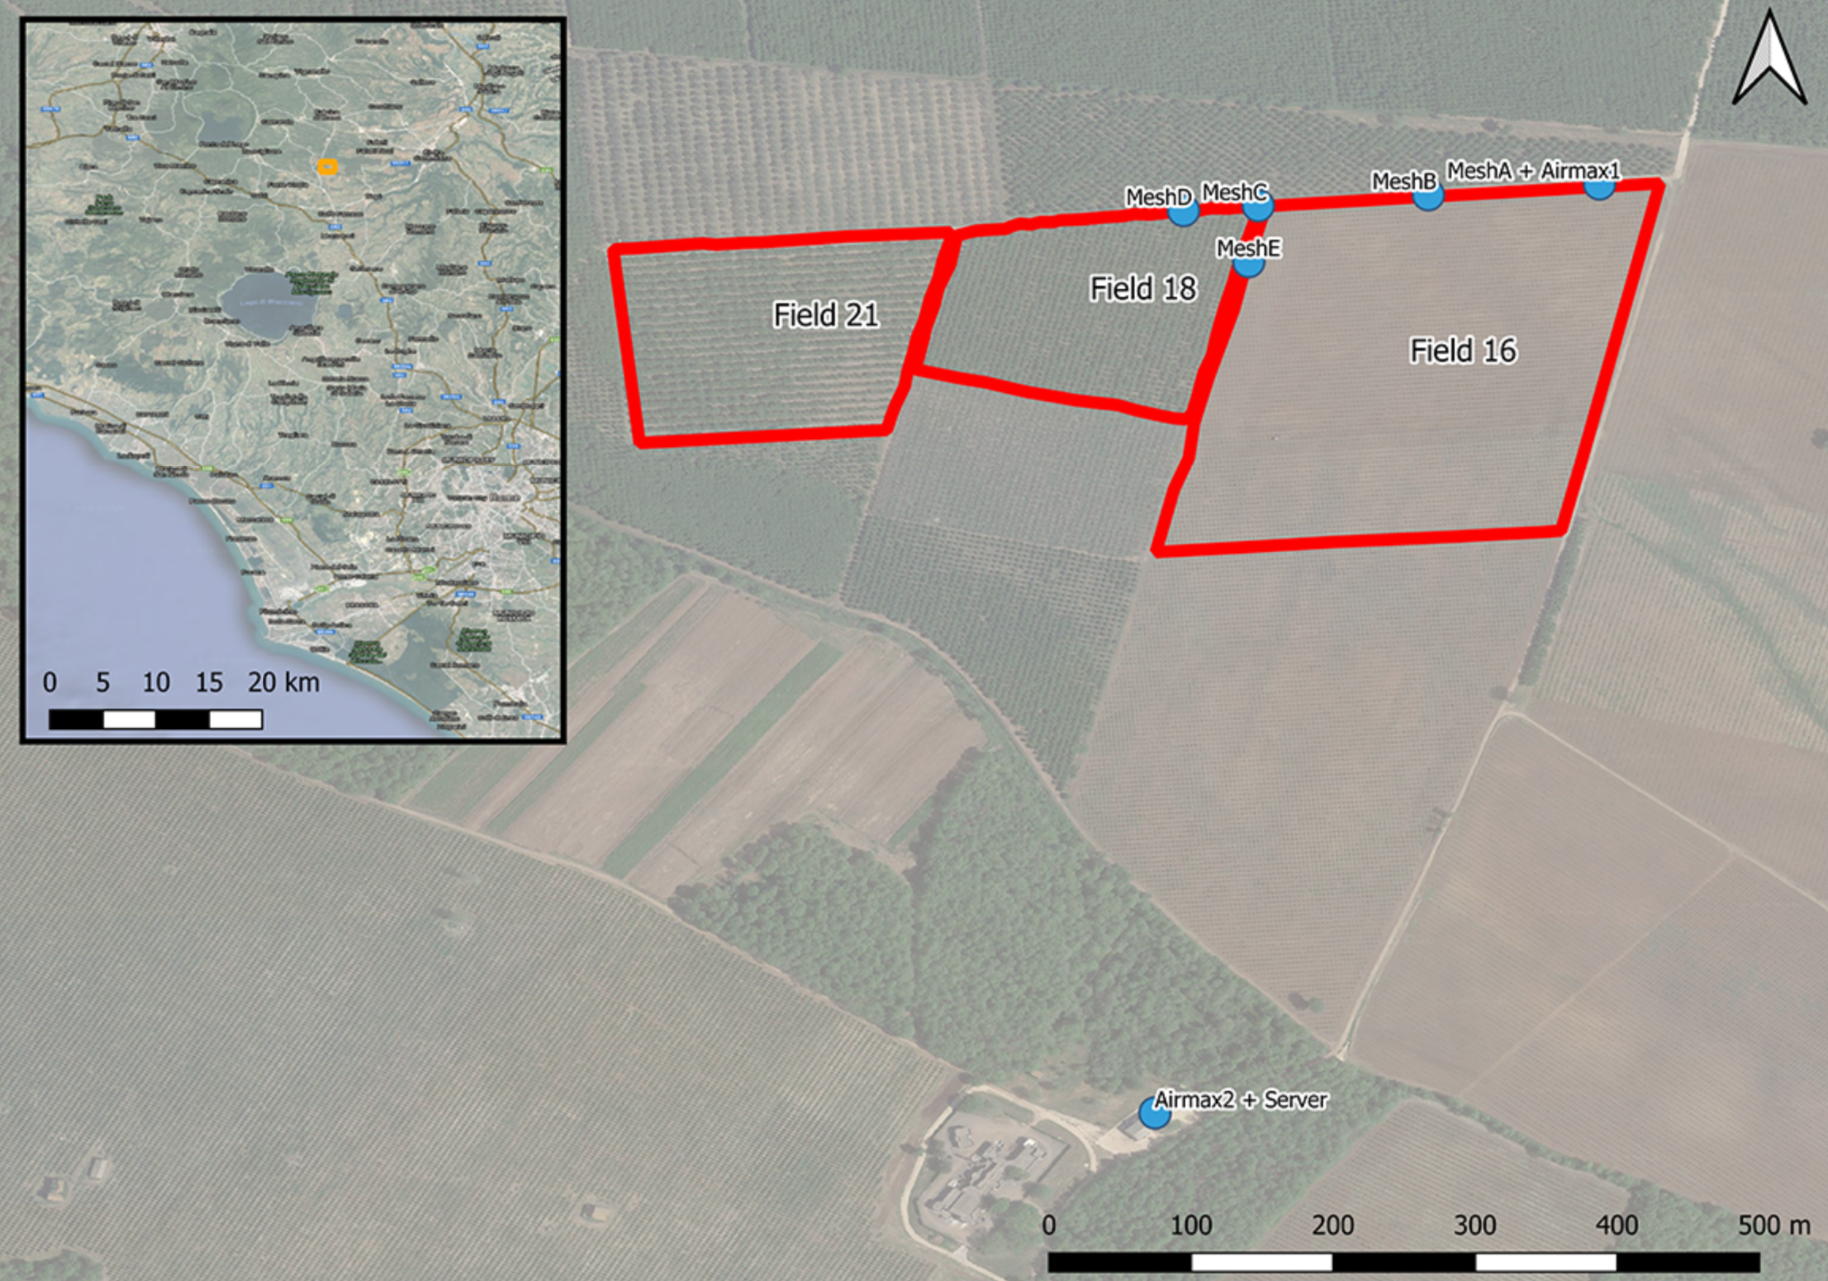
\includegraphics[width=1\textwidth]{selected_fields}
\caption{Noccioleti selezionati per le sperimentazioni del progetto PANTHEON}
\label{fig:selectedfields}
\end{figure}

I dati a disposizione ai fini del progetto provengono dai due noccioleti in questione. I dati in particolare consistono in due file in formato \textit{csv}, \\
\texttt{pantheon20190612-stazione.csv} e \texttt{pantheon20190612-nodi.csv}.\par

Il primo file in particolare contiene dati climatici raccolti dalla stazione meteo presente nel noccioleto della Azienda Agricola Vignola, mentre il secondo file contiene dai provenienti da 9 sensori installati nel terreno, che raccolgono informazioni relativi alla temperatura e alla quantità di acqua presente nel terreno.\par

Di seguito vengono riportati i campi che compongono il file \\ \texttt{pantheon20190612-stazione.csv}:

\begin{itemize}
  \item \texttt{id\_dato}, che contiene un numero progressivo che identifica univocamente ciascuna riga del file;
  \item \texttt{data\_ora}, contenente l'ora solare in cui sono stati ricevuti i dati della riga in questione;
  \item \texttt{temp1\_media}, valore medio di temperatura registrata (gradi Celsius);
  \item \texttt{temp1\_min}, valore minimo di temperatura registrata (gradi Celsius);
  \item \texttt{temp1\_max}, valore massimo di temperatura registrata (gradi Celsius);
  \item \texttt{temp1\_ur1\_n\_letture}, numero di campioni usati per calcolare la temperatura media, minima e massima;
  \item \texttt{ur1\_media}, valore medio di umidità registrata;
  \item \texttt{ur1\_min}, valore minimo di umidità registrata;
  \item \texttt{ur1\_max}, valore massimo di umidità registrata;
  \item \texttt{pioggia\_mm}, mm di piogga caduta;
  \item \texttt{rad W/mq}, radiazione solare (espressa in W/mq);
  \item \texttt{rad\_n\_letture}, numero di campioni usati per calcolare la radiazione solare (\texttt{rad W/mq});
  \item \texttt{wind\_dir}, direzione del vento;
  \item \texttt{wind\_dir\_n\_letture}, numero di campioni considerati per computare la direzione del vento;
  \item \texttt{wind\_speed\_media}, velocità media del vento; 
  \item \texttt{wind\_speed\_max}, velocità massima del vento;
  \item \texttt{wind\_speed\_n\_letture}, numero di campioni considerati per calcolare la velocità massima e media del vento;
  \item \texttt{pressione\_mbar}, pressione atmosferica (in mbar);
  \item \texttt{pressione\_standard\_mbar}, pressione atmosferica corretta al livello del mare (in mbar);
  \item \texttt{pressione\_n\_letture}, numero di campioni impiegati per calcolare la pressione atmosferica (in mbar);
  \item \texttt{rad W/mq array}, elenco dei valori di radiazione al minuto acquisiti durante l’intervallo di acquisizione.
\end{itemize}

Si riportano ora i campi che compongono il file \\ \texttt{pantheon20190612-nodi.csv}:

\begin{itemize}
  \item \texttt{id\_dato}, che contiene un numero progressivo che identifica univocamente ciascuna riga del file;
  \item \texttt{data\_ora}, contenente l'ora solare in cui sono stati ricevuti i dati della riga in questione;
  \item \texttt{soil\_0\_water\_media}, quantità d'acqua presente nel terreno a 15 cm di profondità (espressa in termini percentuali);
  \item \texttt{soil\_0\_water\_n\_letture}, numero di campioni usati per calcolare quantità di acqua nel terreno a 15 cm di profondità;
  \item \texttt{soil\_0\_temp\_media}, valore medio di temperatura del terreno a 15 cm di profondità (gradi celsius);
  \item \texttt{soil\_0\_temp\_n\_letture}, numero di campioni usati per calcolare la temperatura del suolo a 15 cm di profondità;
  \item \texttt{soil\_1\_water\_media}, quantità d'acqua presente nel terreno a 40 cm di profondità (espressa in termini percentuali);
  \item \texttt{soil\_1\_water\_n\_letture}, numero di campioni usati per calcolare quantità di acqua nel terreno a 40 cm di profondità;
  \item \texttt{soil\_1\_temp\_media}, valore medio di temperatura del terreno a 40 cm di profondità (gradi celsius);
  \item \texttt{soil\_1\_temp\_n\_letture}, numero di campioni usati per calcolare la temperatura del suolo a 40 cm di profondità;
\end{itemize}

In particolare i dati registrati dalla stazione meteo vanno dal 12-10-2018 al 12-06-2019.\par
I dati registrati per i vari nodi/sensori invece variano a seconda del nodo:

\begin{itemize}
    \item per il nodo 1 e 2 vanno dal 29-01-2019 al 12-06-2019;
    \item per il nodo 3 vanno dal 18-01-2019 al 03-06-2019;
    \item per il nodo 4, 5, 7, 8, 9 e 10 vanno dal 07-05-2019 al 12-06-2019 (notare come non siano presenti dati per il nodo 6)
\end{itemize}{}